% -------------------------------------------------------------------------------------
% Plantilla de un artículo para publicar en la Revista Colombiana de Estadística
% *************************************************************************************
% -------------------------------------------------------------------------------------
% Establecer primero el idioma principal del artículo, por defecto es español; para
% utilizar otro idioma, cambiar el comando "\documentclass{revcoles}" por el comando
% "\documentclass[english]{revcoles}" o por "\documentclass[portuguese]{revcoles}"
% **** --------------------------------------------------------------------------------
\documentclass[report,oneside]{revcoles}
\labeldocument[
university = Universidad del Valle,
faculty = Facultad de Ingeniería,
department = Escuela de Estadística,
program = Programa Académico de Estadística,
subject = Matemáticas para Estadísticos,
city = Cali,
month = 5,
year = 2018]

% -------------------------------------------------------------------------------------
% Espacio reservado para la carga de los paquetes por parte del autor
% **** --------------------------------------------------------------------------------




% //// --------------------------------------------------------------------------------
% -------------------------------------------------------------------------------------
% Espacio reservado para colocar las definiciones especiales por parte del autor
% **** --------------------------------------------------------------------------------




% //// --------------------------------------------------------------------------------
% -------------------------------------------------------------------------------------
% Espacio utilizado para colocar las palabras que necesitan partición silábica
% **** --------------------------------------------------------------------------------
\hyphenation{Colombia mul-ti-va-ria-do pro-ba-bi-li-dad es-ta-dís-ti-ca}
% //// --------------------------------------------------------------------------------
\begin{document}

% -------------------------------------------------------------------------------------
% Espacio reservado para ingresar el título del artículo
% "maintitle = " título original del artículo
% "secondtitle = " título del artículo traducido al idioma alterno
% "shorttitle = " título corto (opcional) para el encabezado
% **** --------------------------------------------------------------------------------
\title[maintitle = Aproximación de integrales por el método de Simpson,
       %secondtitle = Template for report in a course,
       shorttitle = Método de Simpson
]
% //// --------------------------------------------------------------------------------
% -------------------------------------------------------------------------------------
% Espacio reservado para ingresar el(los) autor(es) del artículo de forma individual.
% opción "firstname = " nombres completos de cada autor
% opción "surname = " primer apellido de cada autor
% opción "numberinstitution = " número que identifica la institución a la que pertenece
%         el autor, en caso de haber solo una institución el campo se elimina
% opción "affiliation = " afiliación o cargo que desempeña el autor en la institución
% opción "email = " dirección electrónica del autor (preferiblemente institucional)
% **** --------------------------------------------------------------------------------
\begin{authors}
\author[firstname = Kevin Steven,
        surname = García,
        code = Código: 1533173,
        email = kevin.chica@correounivalle.edu.co,
]
\author[firstname = Alejandro,
        surname = Soto,
        code = Código: 1532457,
        email = soto.alejandro@correounivalle.edu.co
]
\author[firstname = Bryan,
        surname = Martinez,
        code = Código: 15,
        email = @correounivalle.edu.co,
]
\end{authors}
% //// --------------------------------------------------------------------------------
% -------------------------------------------------------------------------------------
% Espacio reservado para ingresar la información de la(s) institución(es) a la(s)
% cual(es) pertenece(n) el(los) autor(es)
% Usar un comando "\institute"  por cada una de las diferentes instituciones.
% Los campos "subdivision" y "division" son opcionales
% Los campos "institution", "city" y "country" son obligatorios
% **** --------------------------------------------------------------------------------
\begin{comment}
\begin{institutions}
     \institute[subdivision = Departamento de Estadística,
                division = Facultad de Ciencias,
                institution = Universidad del Valle,
                city = Cali,
                country = Colombia]
\end{institutions}
\end{comment}
% //// --------------------------------------------------------------------------------
% -------------------------------------------------------------------------------------
% CUERPO DEL DOCUMENTO
% **** --------------------------------------------------------------------------------
% -------------------------------------------------------------------------------------
% Espacio reservado para colocar el resumen en el idioma principal y las palabras clave
% !!No dejar salto de línea entre el resumen y el comando \keywords{.}¡¡
% **** --------------------------------------------------------------------------------
\begin{comment}
\begin{mainabstract}
Este documento contiene las instrucciones de presentación de los
trabajos de cursos. Este texto está escrito utilizando \LaTeX\
como editor según formato adjunto (archivo \emph{Template for Report.tex})
y puede utilizarse como guía, reemplazando este contenido. Se requieren los
archivos \emph{revcoles.cls}, \emph{references.bib} y \emph{graph\_example.eps}.%
%
\keywords{Formato en \LaTeX\ para documentos, carrera de Estadística}
\end{mainabstract}
\end{comment}
% //// --------------------------------------------------------------------------------
% -------------------------------------------------------------------------------------
% Espacio reservado para colocar el resumen en el idioma secundario y las palabras clave
% !!No dejar salto de línea entre el resumen y el comando \keywords{.}¡¡
% **** --------------------------------------------------------------------------------
\begin{comment}
\begin{secondaryabstract}
This document gives the instructions to prepare a \LaTeX\ version of the graduation project of undergraduate in
Statistics to first semester of 2008. The document is written using a \LaTeX\ format (file \emph{Plantilla para trabajo
de grado.tex}) and can be used as a guideline just replacing its contents. It is necessary to use also the files
\emph{revcoles.cls}, \emph{references.bib} and \emph{graph\_example.eps}.
%
\keywords{\LaTeX\ format for documents, undergraduate in Statistics}
\end{secondaryabstract}

\end{comment}% //// --------------------------------------------------------------------------------
% -------------------------------------------------------------------------------------
% Título de la primera sección
% **** --------------------------------------------------------------------------------
\section{Introducción}
~\\En análisis numérico, la integración numérica constituye una amplia gama de algoritmos para calcular el valor exacto de una integral definida y, por extensión, el término se usa a veces para describir algoritmos numéricos para resolver ecuaciones diferenciales.
~\\El problema básico considerado por la integración numérica es calcular una solución aproximada a la integral definida:
$$\int\limits^{b}_{a}f(x)dx$$
~\\Este problema también puede ser enunciado como un problema de valor inicial para una ecuación diferencial ordinaria, como sigue:
\begin{center}
$y'(x)=f(x)$,  $y(a)=0$
\end{center}
~\\Encontrar $y(b)$ es equivalente a calcular la integral.

~\\Hay varias razones para llevar a cabo la integración numérica. La principal puede ser la imposibilidad de realizar la integración de forma analítica. Es decir, integrales que requerirían de un gran conocimiento y manejo de matemática avanzada, pueden ser resueltas de una manera más sencilla mediante métodos numéricos. Incluso existen funciones integrables pero cuya primitiva no puede ser calculada, siendo la integración numérica de vital importancia. La solución analítica de una integral nos arrojaría una solución exacta, mientras que la solución numérica nos daría una solución aproximada. El error de la aproximación, que depende del método que se utilice y de qué tan fino sea, puede llegar a ser tan pequeño que es posible obtener un resultado idéntico a la solución analítica en las primeras cifras decimales.

~\\Los métodos de integración numérica pueden ser descritos generalmente como combinación de evaluaciones del integrando para obtener una aproximación a la integral. Una parte importante del análisis de cualquier método de integración numérica es estudiar el comportamiento del error de aproximación como una función del número de evaluaciones del integrando. Un método que produce un pequeño error para un pequeño número de evaluaciones es normalmente considerado superior. Reduciendo el número de evaluaciones del integrando se reduce el número de operaciones aritméticas involucradas, y por tanto se reduce el error de redondeo total. También, cada evaluación cuesta tiempo, y el integrando puede ser arbitrariamente complicado.

~\\Existen varios métodos para tratar de llegar al resultado de la integral planteada de forma aproximada, los más utilizados por su simpleza y por su eficiencia son:
\begin{itemize}
\item Regla del rectángulo.
\item Regla del punto medio.
\item Regla del Trapecio.
\item Regla de Simpson.
\end{itemize}

~\\Nosotros nos enfocaremos en desarrollar y mostrar algunos ejemplos de la regla de Simpson.

\section{Método de Simpson}
~\\En este método, se aproxima la integral de f por el área encerrada bajo un arco de parábola que coincide con f en tres puntos: los extremos del intervalo [a, b] y su punto medio:
\begin{center}
\begin{figure}[h]
  \centering
  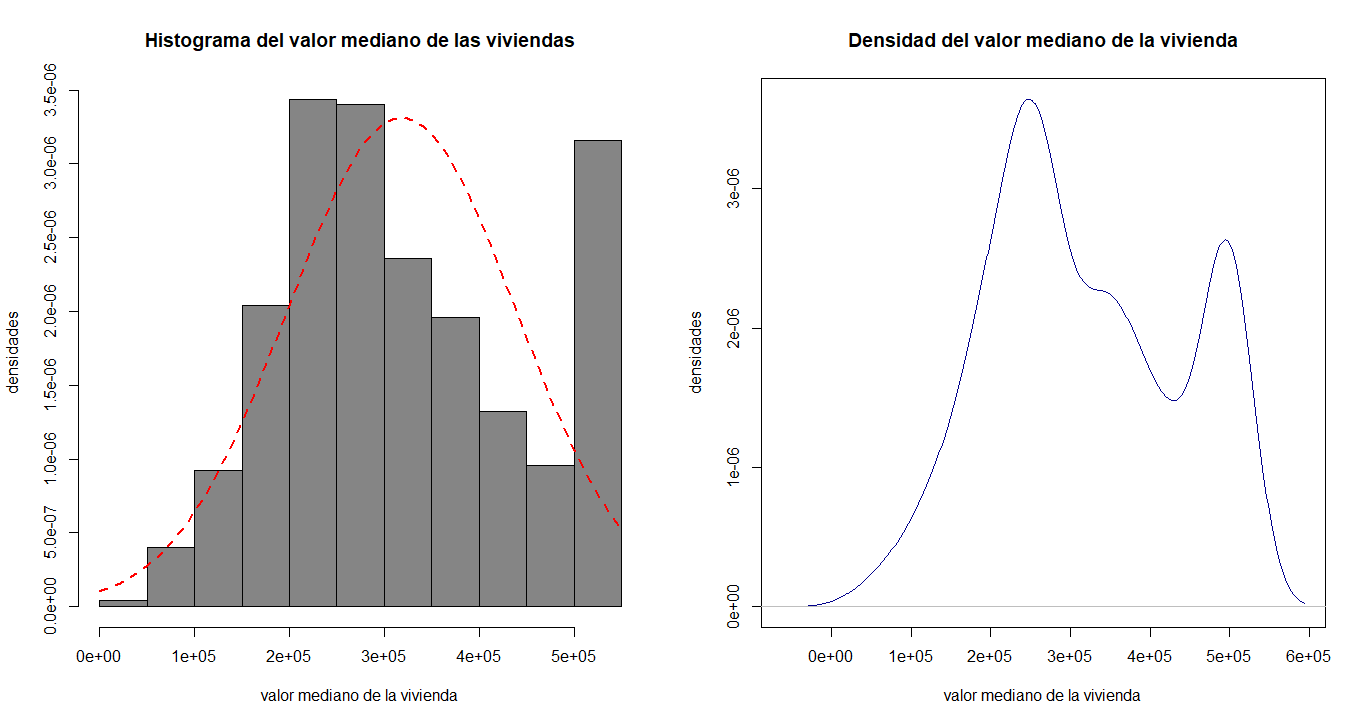
\includegraphics[scale=0.39]{FigurasUV/1.png}
  \caption{Fórmula de Simpson: área bajo la parábola que coincide con f en a, b y $c=\frac{a+b}{2}$}\label{figura1}
\end{figure}
\end{center}

~\\La aproximación está dada por:
$$\int\limits^{b}_{a}f(x)dx \approx \frac{b-a}{6}\left(f(a)+4f\left(\frac{a+b}{2}\right)+f(b)\right)$$

\section{Ejemplos}
\begin{itemize}
\item[]Ejemplo 1: Considere la función $f(x)=cos(2x)$ y halle la integral $\int\limits^{1}_{0} f(x)dx$.
~\\ La integral exacta de forma analítica es:
$$I(f)=\int\limits_{0}^{1}cos(2x)dx=\frac{1}{2}sen(2)=0.4546$$ 
~\\ La idea de acerlo de forma analitica es poder comparar que tan buena es la aproximación.
~\\ Utilizando el método de Simpson, la integral se resuelve de la siguiente manera:
$$I(f)=\int\limits_{0}^{1}cos(2x)dx \approx \frac{1}{6}(cos(0)+4cos(1)+cos(2))=0.4575$$
\item[]Ejemplo 2: Aplicar la regla de Simpson para aproximar la integral $\int\limits_{0}^{1}e^{x^2}dx$
~\\El valor exacto de esta integral es:
$$I(f)=\int\limits_{0}^{1}e^{x^2}dx=1.462651$$ 
~\\ Utilizando el método de Simpson, la integral se resuelve de la siguiente manera:
$$I(f)=\int\limits_{0}^{1}e^{x^2}dx \approx \frac{1}{6}(e^{0}+4 e^{(1/2)^2}+e^{1})=1.475730$$

\end{itemize}


\section{Regla de Simpson compuesta}
~\\Para cualquier regla interpoladora, se puede hacer una aproximación más precisa dividiendo el intervalo $[a,b]$ en algún número n de subintervalos, hallando una aproximación para cada subintervalo, y finalmente sumando todos los resultados. Las reglas que surgen de hacer esto se llaman reglas compuestas, y se caracterizan por perder un orden de precisión global frente a las correspondientes simples, si bien globalmente dan valores más precisos de la integral, a costa eso sí de incrementar significativamente el coste operativo del método.
$$\int\limits_{a}^{b}f(x)dx \approx I^{c}(f)=\sum\limits_{i=1}^{n-1}I(f;[x_{i},x_{i+1}])=\sum\limits_{i=1}^{n-1}\frac{(x_{i+1}-x_{i})}{6}\left(f(x_{i})+4f\left(\frac{x_{i}+x_{i+1}}{2} \right)+f(x_{i+1})\right)$$

~\\En el caso de sub-intervalos de igual longitud, se transforma en:

$$I^{c}(f)=\sum\limits_{i=1}^{n-1}\frac{h}{6}\left(f(x_{i})+4f\left(\frac{x_{i}+x_{i+1}}{2}\right)+f(x_{i+1})\right)=\frac{h}{6}\sum\limits_{i=1}^{n-1}\left(f(x_{i})+4f\left(\frac{x_{i}+x_{i+1}}{2}\right)+f(x_{i+1})\right)$$

$$=\frac{h}{6}\left\lbrace f(x_{1})+2\sum\limits_{i=2}^{n-1}f(x_{i})+f(x_{n})+4\sum\limits_{i=1}^{n-1}f\left(\frac{x_{i}+x_{i+1}}{2}\right)\right\rbrace$$
~\\donde $h=\frac{b-a}{n}$.
\section{Ejemplos}
\begin{itemize}
\item[]Ejemplo 1: Se considera de nuevo la integral del ejemplo 1 de la sección anterior:
$$I(f)=\int\limits_{0}^{1}cos(2x)dx=\frac{1}{2}sen(2)=0.4546$$
~\\Utilizando la fórmula de Simpson compuesta con 5 sub-intervalos de igual longitud (es decir, $h=\frac{b-a}{n}=\frac{1}{5}=0.2$ y $\left\lbrace x_{i} \right\rbrace ^{6}_{i=1}=\left\lbrace 0,0.2,0.4,0.6,0.8,1 \right\rbrace )$, se obtiene:

$$I^{c}(f)=\frac{h}{6}\sum\limits_{i=1}^{5} \left( cos(2x_{i})+4cos \left( 2\frac{x_{i}+x_{i+1}}{2} \right)+cos(2x_{i+1}) \right)$$

$$=0.03333\{ cos(0)+2(cos(0.4)+cos(0.8)+cos(1.2)+cos(1.6))+cos(2)$$
$$+4(cos(0.2)+cos(0.6)+cos(1)+cos(1.4)+cos(1.8))\}=0.4546$$

\item[]Ejemplo 2: Se considera de nuevo la integral del ejemplo 2 de la sección anterior:
$$I(f)=\int\limits_{0}^{1}e^{x^2}dx=1.462651$$ 
~\\Utilizando la fórmula de Simpson compuesta con 5 sub-intervalos de igual longitud (es decir, $h=\frac{b-a}{n}=\frac{1}{5}=0.2$ y $\left\lbrace x_{i} \right\rbrace ^{6}_{i=1}=\left\lbrace 0,0.2,0.4,0.6,0.8,1 \right\rbrace )$, se obtiene:

$$I^{c}(f)=\frac{h}{6}\sum\limits_{i=1}^{5} \left( e^{x^{2}_{i}}+4 e^{\left(\frac{x_{i}+x_{i+1}}{2} \right)^2}+e^{x_{i+1}^2} \right)$$

$$=0.03333\left\lbrace e^{0}+2(e^{0.2^2}+e^{0.4^2}+e^{0.6^2}+e^{0.8^2})+e^{1^2}+4(e^{0.1^2}+e^{0.3^2}+e^{0.5^2}+e^{0.7^2}+e^{0.9^2})\right\rbrace$$
$$=0.03333(43.880442)=1.462682$$
\end{itemize}



% //// --------------------------------------------------------------------------------
% -------------------------------------------------------------------------------------
% Fin del cuerpo del documento
% **** --------------------------------------------------------------------------------
% **** --------------------------------------------------------------------------------
% Espacio para colocar el nombre del archivo *.bib (sin la extensión .bib) que contiene
% las referencias bibliográficas del artículo utilizando el estilo bibliográfico BibTeX
% "\referencias{.}"
% **** --------------------------------------------------------------------------------
\bibliography{references}
% //// --------------------------------------------------------------------------------
% //// --------------------------------------------------------------------------------
    \appendix% !no modificar esta línea¡
% -------------------------------------------------------------------------------------
% Espacio para ubicar los apéndices: tablas y gráficas
% **** --------------------------------------------------------------------------------


% -------------------------------------------------------------------------------------
% Fin del artículo
% **** --------------------------------------------------------------------------------
\end{document}
